\chapter{Training Optimization}
\label{chap:training_optimization}

\begin{tldr}
Training optimization is where theory meets practice. This chapter covers optimizers (SGD, Adam, AdamW), learning rate schedules, batch size scaling, mixed precision training, gradient problems and solutions, regularization, and distributed training. These topics come up in every ML interview---you need to explain trade-offs, make practical recommendations, and debug training failures. If you can only master one chapter before an interview, make it this one.
\end{tldr}

%==============================================================================
\section{Optimizers}
\label{sec:optimizers}
%==============================================================================

The optimizer determines \textit{how} you update parameters given the gradient. Every optimizer is some variation of: compute a direction, scale it, step in that direction.

\subsection{SGD with Momentum}

\textbf{What it is.} Vanilla SGD updates are noisy and slow. Momentum accumulates a running average of past gradients, smoothing out oscillations and accelerating convergence in consistent directions---like a heavy ball rolling down a hill.

\begin{mathresult}{SGD with Momentum}
\begin{align}
\vv_t &= \beta \vv_{t-1} + \nabla_\theta \loss(\theta_{t-1}) \\
\theta_t &= \theta_{t-1} - \eta \vv_t
\end{align}
where $\eta$ is the learning rate and $\beta$ (typically $0.9$) is the momentum coefficient.

\textbf{Nesterov variant:} Compute gradient at the \emph{lookahead} position $\theta - \eta \beta \vv_{t-1}$, giving a corrective effect that reduces overshooting.
\end{mathresult}

\textbf{When to use.} Vision tasks (ResNets, ConvNeXt), settings where you want maximum generalization and are willing to tune the learning rate carefully.

\textbf{Pitfalls.} Requires careful LR tuning and a good schedule. Without a schedule, momentum SGD often stalls at saddle points.

\subsection{Adam}

\textbf{What it is.} Adam combines momentum (first moment) with per-parameter adaptive learning rates (second moment). Each parameter gets its own effective learning rate based on the history of its gradients: parameters with consistently large gradients get smaller steps, and vice versa.

\begin{mathresult}{Adam Update Rule}
\begin{align}
m_t &= \beta_1 m_{t-1} + (1 - \beta_1) g_t & \text{(first moment: momentum)} \\
v_t &= \beta_2 v_{t-1} + (1 - \beta_2) g_t^2 & \text{(second moment: scale)} \\
\hat{m}_t &= m_t / (1 - \beta_1^t) & \text{(bias correction)} \\
\hat{v}_t &= v_t / (1 - \beta_2^t) & \text{(bias correction)} \\
\theta_t &= \theta_{t-1} - \eta \cdot \hat{m}_t / (\sqrt{\hat{v}_t} + \epsilon)
\end{align}
Defaults: $\beta_1 = 0.9$, $\beta_2 = 0.999$, $\epsilon = 10^{-8}$.
\end{mathresult}

\textbf{Bias correction in one sentence:} Since $m_0 = v_0 = 0$, the early estimates are biased toward zero; dividing by $(1 - \beta^t)$ corrects this. The correction matters most in the first few hundred steps and becomes negligible as $t$ grows.

\textbf{When to use.} NLP tasks, transformers, GANs, any setting where you want fast convergence with less LR tuning. Adam is the default starting point for most deep learning.

\textbf{Pitfalls.} Can generalize worse than SGD on vision tasks. The adaptive learning rate can interact poorly with weight decay (see AdamW below).

\subsection{AdamW: Decoupled Weight Decay}

\textbf{What it is.} The critical fix to Adam's handling of weight decay. In standard Adam, L2 regularization is added to the loss gradient \textit{before} the adaptive scaling, which means the regularization gets divided by $\sqrt{v_t}$---effectively reducing weight decay for parameters with large gradients (the ones that need it most). AdamW applies weight decay \textit{directly} to the parameters, bypassing the adaptive scaling.

\begin{keyinsight}{AdamW Decouples Weight Decay from the Adaptive Gradient}
In SGD, L2 regularization and weight decay are mathematically equivalent:
\begin{equation}
\nabla_\theta(\loss + \tfrac{\lambda}{2}\|\theta\|^2) = \nabla_\theta \loss + \lambda\theta
\end{equation}
In Adam, they are \textbf{not} equivalent because the adaptive scaling $1/\sqrt{v_t}$ modifies the regularization gradient differently from the loss gradient. AdamW restores the intended behavior by decoupling:
\begin{equation}
\theta_t = \theta_{t-1} - \eta\left(\frac{\hat{m}_t}{\sqrt{\hat{v}_t} + \epsilon} + \lambda \theta_{t-1}\right)
\end{equation}
\end{keyinsight}

\textbf{When to use.} Always use AdamW instead of Adam when you want weight decay. This is the default optimizer for LLM training (GPT, LLaMA, etc.).

\subsection{LAMB and LARS}

\textbf{LARS} (Layer-wise Adaptive Rate Scaling): Scales the learning rate per layer by the ratio of parameter norm to gradient norm. Designed for large-batch training of CNNs (e.g., batch size 8K--32K).

\textbf{LAMB} (Layer-wise Adaptive Moments): The Adam equivalent of LARS. Combines Adam's adaptive moments with LARS-style layer-wise scaling. Used for large-batch BERT pretraining.

\textbf{One-sentence summary:} LARS and LAMB normalize the update per layer so that no single layer dominates, which stabilizes large-batch training.

\subsection{Optimizer Comparison}

\begin{table}[H]
\centering
\caption{Optimizer comparison: when to use each}
\begin{tabularx}{\textwidth}{lXXX}
\toprule
\textbf{Optimizer} & \textbf{Best For} & \textbf{Key Hyperparameters} & \textbf{Notes} \\
\midrule
SGD + Momentum & Vision (ResNet, ConvNeXt) & LR, momentum (0.9), schedule & Best generalization when well-tuned \\
Adam & Fast prototyping, NLP, GANs & LR ($3\mathrm{e}{-4}$), $\beta_1$, $\beta_2$ & Less LR-sensitive, faster convergence \\
AdamW & LLMs, Transformers, default & LR, weight decay ($0.01$--$0.1$) & Always prefer over Adam with WD \\
LAMB/LARS & Large-batch training & Trust ratio, warmup & Only needed at batch $\geq$ 4K \\
Adafactor & Memory-constrained LLMs & Factored second moment & Saves memory vs.\ Adam \\
\bottomrule
\end{tabularx}
\end{table}

%==============================================================================
\section{Learning Rate Schedules}
\label{sec:lr_schedules}
%==============================================================================

The learning rate is the single most important hyperparameter. A good schedule can be worth more than a better architecture.

\subsection{Warmup}

\textbf{What it is.} Start with a very small LR and linearly increase to the target LR over the first $T_w$ steps. Stabilizes early training when parameter statistics are far from their converged values.

\textbf{Why it helps.} At initialization, the model's activations and gradients have high variance. Large updates at this stage can push the model into a bad region of the loss landscape from which it never recovers. Warmup gives the optimizer's running statistics (especially Adam's $v_t$) time to calibrate.

\textbf{Typical values.} 1--5\% of total training steps. For LLMs, 2000 steps is a common default.

\subsection{Step Decay}

\textbf{What it is.} Multiply LR by a factor (e.g., 0.1) at predetermined epochs. Simple and effective for CNNs.

\textbf{Example:} Start at $0.1$, multiply by $0.1$ at epochs 30, 60, 90.

\textbf{Limitation.} Requires knowing the right epochs to decay. The abrupt drops can cause training instability.

\subsection{Cosine Annealing}

\begin{mathresult}{Cosine Annealing Schedule}
\begin{equation}
\eta_t = \eta_{\min} + \frac{1}{2}(\eta_{\max} - \eta_{\min})\left(1 + \cos\left(\frac{t}{T}\pi\right)\right)
\end{equation}
where $T$ is the total number of steps, $\eta_{\max}$ is the peak LR, and $\eta_{\min}$ is the final LR (often $0$ or $0.1 \times \eta_{\max}$).
\end{mathresult}

\textbf{Why it works.} Smooth decay avoids the shock of step decay. Spends more time at moderate LRs (the ``useful'' range), and the slow final decay lets the model settle into a good minimum.

\subsection{Warmup + Cosine Decay: The Modern Default}

For Transformers and LLMs, the standard schedule is:
\begin{enumerate}
    \item \textbf{Linear warmup} for $T_w$ steps (LR from 0 to $\eta_{\max}$)
    \item \textbf{Cosine decay} for remaining steps (LR from $\eta_{\max}$ to $\eta_{\min}$)
\end{enumerate}

This is what GPT-3, LLaMA, and nearly every modern LLM uses. If you only remember one schedule, remember this one.

\subsection{Schedule Comparison}

\begin{table}[H]
\centering
\caption{Learning rate schedule comparison}
\begin{tabularx}{\textwidth}{lXXl}
\toprule
\textbf{Schedule} & \textbf{Description} & \textbf{Use Case} & \textbf{Modern?} \\
\midrule
Step decay & Multiply by factor at fixed epochs & CNNs (ResNet) & Legacy \\
Cosine annealing & Smooth cosine from peak to min & General training & Yes \\
Warmup + cosine & Linear warmup then cosine decay & LLMs, Transformers & Standard \\
One-cycle & Warmup to high LR, then decay to near zero & Fast training & Niche \\
Inverse sqrt & $\eta_t = \eta_0 / \sqrt{t}$ & Original Transformer & Legacy \\
\bottomrule
\end{tabularx}
\end{table}

\subsection{LR Schedule Shapes}

\begin{figure}[H]
\centering
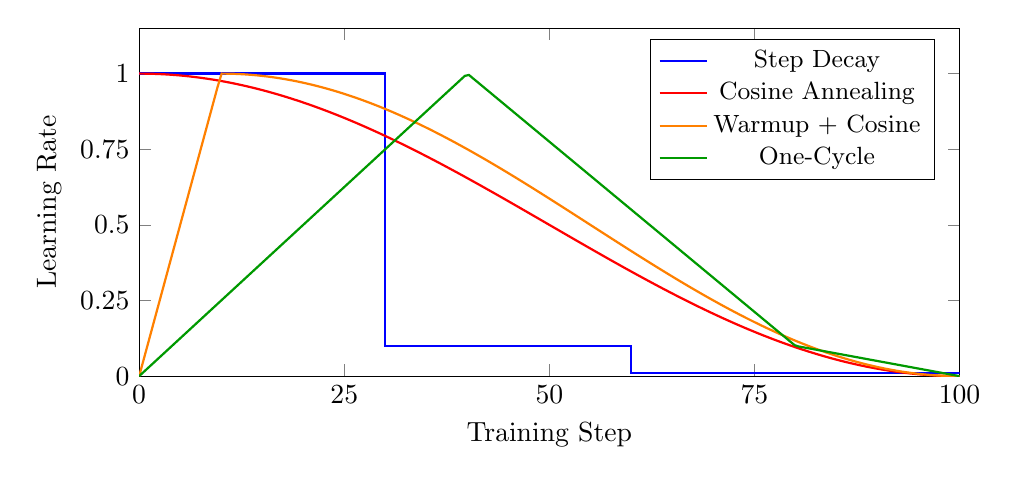
\begin{tikzpicture}
    \begin{axis}[
        xlabel={Training Step},
        ylabel={Learning Rate},
        xmin=0, xmax=100,
        ymin=0, ymax=1.15,
        width=12cm,
        height=6cm,
        legend pos=north east,
        legend style={font=\small},
        xtick={0,25,50,75,100},
        ytick={0,0.25,0.5,0.75,1.0}
    ]
    % Step decay
    \addplot[thick, blue, const plot] coordinates {
        (0,1.0) (30,1.0) (30,0.1) (60,0.1) (60,0.01) (100,0.01)
    };
    \addlegendentry{Step Decay}

    % Cosine annealing
    \addplot[domain=0:100, samples=200, thick, red] {0.5*(1+cos(deg(x/100*pi)))};
    \addlegendentry{Cosine Annealing}

    % Warmup + cosine
    \addplot[thick, orange, samples=200, domain=0:100]
        {x < 10 ? x/10 : 0.5*(1+cos(deg((x-10)/90*pi)))};
    \addlegendentry{Warmup + Cosine}

    % One-cycle
    \addplot[thick, green!60!black, samples=200, domain=0:100]
        {x < 40 ? x/40 : (x < 80 ? 1 - (x-40)/40*0.9 : 0.1 - (x-80)/20*0.1)};
    \addlegendentry{One-Cycle}

    \end{axis}
\end{tikzpicture}
\caption{Common learning rate schedule shapes. Warmup + cosine decay is the modern default for Transformer training.}
\label{fig:lr_schedules}
\end{figure}

%==============================================================================
\section{Batch Size and Learning Rate Scaling}
\label{sec:batch_scaling}
%==============================================================================

\subsection{The Linear Scaling Rule}

\textbf{What it is.} When you increase the batch size by a factor $k$, you should also increase the learning rate by $k$. The intuition: a larger batch gives a more accurate gradient estimate, so you can take a proportionally larger step.

\begin{mathresult}{Linear Scaling Rule}
\begin{equation}
\eta_{\text{new}} = \eta_{\text{base}} \times \frac{B_{\text{new}}}{B_{\text{base}}}
\end{equation}
If you double the batch size, double the learning rate.
\end{mathresult}

\textbf{When it breaks.} The linear scaling rule fails for very large batches (typically $B > 8\text{K}$ for vision, varies for NLP). At extreme batch sizes, the gradient noise reduction hits diminishing returns, and the larger steps overshoot. This is where warmup and LARS/LAMB become necessary.

\subsection{Gradient Accumulation}

\textbf{What it is.} Simulate a larger batch size without increasing memory. Instead of updating after every mini-batch, accumulate gradients over $k$ mini-batches, then update once. The effective batch size becomes $k \times B$.

\textbf{When to use.} When your GPU memory limits your batch size but you need a larger effective batch (e.g., for contrastive learning, large-batch LLM training, or to match a reference training recipe).

\textbf{Caveat.} Gradient accumulation is \textit{not} identical to a true larger batch for batch normalization, since BatchNorm statistics are still computed per mini-batch. Use GroupNorm or LayerNorm in this scenario.

\subsection{Small Batch vs Large Batch Trade-offs}

\begin{table}[H]
\centering
\caption{Small batch vs large batch trade-offs}
\begin{tabularx}{\textwidth}{lXX}
\toprule
\textbf{Dimension} & \textbf{Small Batch (32--256)} & \textbf{Large Batch (2K--64K)} \\
\midrule
Gradient noise & High (more stochastic) & Low (smoother estimate) \\
Generalization & Often better (noise acts as regularizer) & Can be worse (sharp minima) \\
Throughput & Lower GPU utilization & Higher GPU utilization \\
Memory & Lower per GPU & Higher per GPU \\
LR sensitivity & Less sensitive & More sensitive; needs warmup \\
Convergence speed & More parameter updates per epoch & Fewer updates but more data per update \\
Training wall-time & Longer (if GPU is underutilized) & Shorter (better parallelism) \\
\bottomrule
\end{tabularx}
\end{table}

\textbf{The practical answer.} Use the largest batch that fits in memory, apply the linear scaling rule, and add warmup. If generalization degrades at very large batches, consider techniques like LARS/LAMB or stochastic weight averaging (SWA).

%==============================================================================
\section{Mixed Precision Training}
\label{sec:mixed_precision}
%==============================================================================

\textbf{What it is.} Perform most computations (forward pass, backward pass) in half precision (FP16 or BF16) while keeping a master copy of weights in FP32. This roughly doubles training speed and halves memory for activations, with negligible accuracy loss.

\textbf{How it works:}
\begin{enumerate}
    \item Maintain FP32 master weights
    \item Cast to FP16/BF16 for forward and backward pass
    \item Compute gradients in half precision
    \item Update FP32 master weights (accumulate in full precision to avoid rounding errors)
\end{enumerate}

\subsection{Loss Scaling}

\textbf{Why.} FP16 has limited dynamic range. Small gradients (common in deep networks) can underflow to zero. Loss scaling multiplies the loss by a large factor before backward, amplifying gradients into the representable range, then divides the gradients by the same factor before the optimizer step.

\textbf{How.} Dynamic loss scaling (PyTorch default): start with a large scale factor (e.g., $2^{16}$), reduce it if gradients overflow (NaN/Inf), increase it periodically if training is stable.

\subsection{FP16 vs BF16}

\begin{table}[H]
\centering
\caption{FP16 vs BF16 for training}
\begin{tabularx}{\textwidth}{lXX}
\toprule
\textbf{Property} & \textbf{FP16} & \textbf{BF16} \\
\midrule
Exponent bits & 5 & 8 (same as FP32) \\
Mantissa bits & 10 & 7 \\
Dynamic range & $\sim 6 \times 10^{4}$ & $\sim 3.4 \times 10^{38}$ (same as FP32) \\
Precision & Higher (more mantissa bits) & Lower \\
Loss scaling & Required & Usually not needed \\
Hardware & All modern GPUs & A100+, TPUs \\
Best for & Inference, older GPUs & LLM training \\
\bottomrule
\end{tabularx}
\end{table}

\begin{warningbox}
BF16 is almost always preferred over FP16 for LLM training. FP16's limited dynamic range causes gradient underflow in deep networks, requiring careful loss scaling. BF16 has the same range as FP32, so gradients rarely underflow. If your hardware supports BF16, use it.
\end{warningbox}

%==============================================================================
\section{Gradient Problems and Solutions}
\label{sec:gradient_problems}
%==============================================================================

\subsection{Vanishing Gradients}

\textbf{What it is.} Gradients shrink exponentially as they propagate backward through many layers. After $L$ layers with Jacobian spectral norm $< 1$, the gradient magnitude scales as $\sim \rho^L$ where $\rho < 1$. Early layers receive near-zero gradients and stop learning.

\textbf{Causes:}
\begin{itemize}
    \item Deep networks without residual connections
    \item Saturating activations (sigmoid, tanh) that squash gradients to near-zero
    \item Long sequences in RNNs (BPTT over many timesteps)
    \item Poor weight initialization (too-small initial weights)
\end{itemize}

\textbf{Solutions:}

\begin{table}[H]
\centering
\caption{Solutions for vanishing gradients}
\begin{tabularx}{\textwidth}{lX}
\toprule
\textbf{Solution} & \textbf{How It Helps} \\
\midrule
Residual connections & Gradient flows directly through skip connections ($\partial \loss / \partial \vx$ includes an identity term) \\
Non-saturating activations & ReLU, GELU, SiLU have gradient $\approx 1$ for positive inputs \\
Proper initialization & He init for ReLU; Xavier for tanh/sigmoid; keeps gradient variance $\approx 1$ per layer \\
Normalization layers & LayerNorm / BatchNorm re-center and re-scale activations, preventing drift \\
LSTM/GRU gates & Gating mechanism allows gradients to flow unimpeded through the cell state \\
\bottomrule
\end{tabularx}
\end{table}

\subsection{Exploding Gradients}

\textbf{What it is.} The opposite problem: gradients grow exponentially through layers ($\rho > 1$), causing parameter updates so large they destroy the model. You typically see NaN losses or sudden loss spikes.

\textbf{Solution: Gradient Clipping.} Cap the gradient norm before the optimizer step.

\begin{mathresult}{Gradient Norm Clipping}
\begin{equation}
\hat{g} = \begin{cases}
g & \text{if } \|g\| \leq c \\
c \cdot \frac{g}{\|g\|} & \text{if } \|g\| > c
\end{cases}
\end{equation}
Typical threshold: $c = 1.0$ for LLMs, $c = 5.0$ for RNNs.
\end{mathresult}

\textbf{Norm clipping vs.\ value clipping.} Norm clipping preserves the direction of the gradient (only scales magnitude). Value clipping clips each element independently, which can change the direction. Always prefer norm clipping.

\subsection{Gradient Checkpointing}

\textbf{What it is.} A memory-compute trade-off. Instead of storing all intermediate activations for the backward pass, only store activations at ``checkpoints'' (e.g., every $k$-th layer). During backward, recompute the missing activations on the fly.

\textbf{Trade-off:}
\begin{itemize}
    \item \textbf{Memory savings:} From $O(L)$ to $O(\sqrt{L})$ activation memory (with $\sqrt{L}$ checkpoints)
    \item \textbf{Compute cost:} Roughly 30--40\% more compute (one extra forward pass per segment)
\end{itemize}

\textbf{When to use.} Training large models that don't fit in GPU memory, or when you need a larger batch size. Standard practice for LLM training.

\subsection{Loss Curve Diagnostics}

\begin{figure}[H]
\centering
\begin{tikzpicture}
    % Healthy training
    \begin{axis}[
        name=plot1,
        width=5.5cm, height=4cm,
        title={\small Healthy Training},
        xlabel={\tiny Step}, ylabel={\tiny Loss},
        xmin=0, xmax=100, ymin=0, ymax=3,
        xtick=\empty, ytick=\empty,
        title style={font=\small\bfseries}
    ]
    \addplot[thick, blue, smooth, samples=100, domain=0:100] {2.5*exp(-x/25) + 0.2 + 0.05*rand};
    \end{axis}

    % Loss plateau
    \begin{axis}[
        name=plot2,
        at={($(plot1.east)+(1.5cm,0)$)}, anchor=west,
        width=5.5cm, height=4cm,
        title={\small Loss Plateau},
        xlabel={\tiny Step}, ylabel={\tiny Loss},
        xmin=0, xmax=100, ymin=0, ymax=3,
        xtick=\empty, ytick=\empty,
        title style={font=\small\bfseries}
    ]
    \addplot[thick, red, smooth, samples=100, domain=0:100] {2.5*exp(-x/15)*(x<30) + 1.2*(x>=30) + 0.03*rand};
    \end{axis}

    % Oscillating loss
    \begin{axis}[
        name=plot3,
        at={($(plot1.south)-(0,1.8cm)$)}, anchor=north,
        width=5.5cm, height=4cm,
        title={\small Oscillating Loss},
        xlabel={\tiny Step}, ylabel={\tiny Loss},
        xmin=0, xmax=100, ymin=0, ymax=3,
        xtick=\empty, ytick=\empty,
        title style={font=\small\bfseries}
    ]
    \addplot[thick, orange, samples=200, domain=0:100] {1.5 + 0.8*sin(deg(x/3)) + 0.3*rand};
    \end{axis}

    % Loss spike
    \begin{axis}[
        name=plot4,
        at={($(plot2.south)-(0,1.8cm)$)}, anchor=north,
        width=5.5cm, height=4cm,
        title={\small Loss Spike},
        xlabel={\tiny Step}, ylabel={\tiny Loss},
        xmin=0, xmax=100, ymin=0, ymax=4,
        xtick=\empty, ytick=\empty,
        title style={font=\small\bfseries}
    ]
    \addplot[thick, purple, smooth, samples=100, domain=0:100]
        {2.5*exp(-x/25) + 0.2 + (x>45 && x<55 ? 2.5*exp(-(x-50)^2/5) : 0)};
    \end{axis}
\end{tikzpicture}
\caption{Four common loss curve patterns. Each suggests a different debugging action.}
\label{fig:loss_diagnostics}
\end{figure}

\begin{warningbox}
If the loss spikes during training, debug in this order: (1) Check the learning rate---is it too high or did a schedule step trigger? (2) Check the data pipeline---did a corrupted batch slip through? (3) Check gradient norms---are they exploding? Add or reduce gradient clipping. (4) Check for numerical issues---switch to BF16 or add loss scaling.
\end{warningbox}

%==============================================================================
\section{Regularization Techniques}
\label{sec:regularization}
%==============================================================================

Regularization prevents overfitting by constraining model capacity. The right combination of techniques matters more than any single one.

\subsection{Dropout}

\textbf{What it is.} During training, randomly zero out each neuron's output with probability $p$. At inference, use all neurons but scale outputs by $(1-p)$ (or equivalently, scale training outputs by $1/(1-p)$ --- called inverted dropout, which is the standard implementation).

\textbf{Where to apply:}
\begin{itemize}
    \item After fully connected layers: $p = 0.1$--$0.5$
    \item In Transformer attention: $p = 0.1$ (attention dropout)
    \item After residual connections: $p = 0.1$ (Transformer standard)
    \item \textbf{Not} in batch normalization layers (they provide their own regularization)
\end{itemize}

\textbf{Variants:}
\begin{itemize}
    \item \textbf{DropConnect:} Zero out individual weights instead of neurons
    \item \textbf{Spatial Dropout:} Drop entire channels in CNNs (preserves spatial structure)
    \item \textbf{DropPath / Stochastic Depth:} Drop entire residual blocks during training
\end{itemize}

\subsection{Weight Decay}

\textbf{What it is.} Penalize large weights by adding $\lambda\|\theta\|^2$ to the loss (L2) or directly decaying weights each step by factor $(1 - \eta\lambda)$ (decoupled). Prevents any single weight from dominating.

\textbf{Critical distinction.} L2 regularization (add $\lambda\theta$ to the gradient) and decoupled weight decay (subtract $\lambda\theta$ from parameters directly) are equivalent for SGD but \textbf{not equivalent for Adam}. See Section~\ref{sec:optimizers} on AdamW.

\textbf{Typical values:} $\lambda = 0.01$ for AdamW (LLMs), $\lambda = 10^{-4}$ for SGD (vision).

\subsection{Data Augmentation}

\textbf{What it is.} Artificially expand the training set by applying transformations that preserve labels. Widely regarded as the single most effective regularizer for vision tasks.

\textbf{Common techniques:} Random crop, horizontal flip, color jitter, RandAugment, CutMix, MixUp.

\textbf{MixUp} deserves special mention: it trains on convex combinations of input pairs and their labels, smoothing the decision boundary.

\subsection{Stochastic Depth (DropPath)}

\textbf{What it is.} During training, randomly skip entire residual blocks. Each block has a survival probability that decreases linearly from 1.0 (first block) to some minimum (last block, e.g., 0.8). Effectively trains an ensemble of networks with different depths.

\textbf{When to use.} Deep residual networks (100+ layers), Vision Transformers (DeiT uses this), any architecture with residual connections.

\subsection{Early Stopping}

\textbf{What it is.} Monitor validation loss and stop training when it begins to increase. The simplest form of regularization---limit the number of optimization steps.

\textbf{When to use.} Always monitor validation metrics. Use early stopping as a safety net, but prefer explicit regularization (dropout, weight decay) as the primary defense against overfitting.

\subsection{Regularization Comparison}

\begin{table}[H]
\centering
\caption{Regularization technique comparison}
\begin{tabularx}{\textwidth}{lXlX}
\toprule
\textbf{Technique} & \textbf{Mechanism} & \textbf{Typical Values} & \textbf{Use Case} \\
\midrule
Dropout & Zero random neurons & $p = 0.1$--$0.3$ & FC layers, Transformers \\
Weight decay & Penalize large weights & $0.01$--$0.1$ (AdamW) & Always (essentially free) \\
Data augmentation & Transform inputs & Task-specific & Vision (most effective) \\
Stochastic depth & Drop residual blocks & Survival $0.8$--$1.0$ & Deep resnets, ViTs \\
Label smoothing & Soften targets & $\epsilon = 0.1$ & Classification \\
Early stopping & Limit training steps & Patience 5--10 epochs & Safety net \\
\bottomrule
\end{tabularx}
\end{table}

\begin{warningbox}
L2 regularization and weight decay are only equivalent for SGD. In Adam, L2 regularization gets scaled by the adaptive learning rate, weakening it for high-gradient parameters. Always use AdamW (decoupled weight decay) instead of Adam + L2. This is one of the most commonly missed details in interviews.
\end{warningbox}

%==============================================================================
\section{Distributed Training}
\label{sec:distributed}
%==============================================================================

When a model or dataset is too large for a single GPU, you need distributed training. The key question is: \textit{what do you distribute?}

\subsection{Data Parallelism (DDP)}

\textbf{What it is.} Every GPU holds a complete copy of the model. Data is split across GPUs. Each GPU computes gradients on its shard of data, then gradients are synchronized via \texttt{all-reduce} before the optimizer step.

\textbf{How all-reduce works:} In ring all-reduce, each GPU sends a chunk of gradients to the next GPU in a ring. After $2(N-1)$ steps (where $N$ is the number of GPUs), every GPU has the sum of all gradients. Communication cost is $O(\text{model size})$, independent of GPU count.

\textbf{When to use.} The model fits on a single GPU. This is the simplest and most efficient strategy---always start here.

\textbf{Limitation.} Every GPU stores the full model, optimizer states, and gradients. For a 7B model with Adam in FP32, that is $\sim$112 GB per GPU (parameters + gradients + optimizer states).

\subsection{Model Parallelism}

When the model is too large for a single GPU, split it across GPUs.

\textbf{Tensor Parallelism:} Split individual layers across GPUs. For example, split a large matrix multiplication $\mY = \mX\mW$ by partitioning $\mW$ column-wise across GPUs. Each GPU computes part of the output, then results are gathered. Requires high-bandwidth interconnect (NVLink).

\textbf{Pipeline Parallelism:} Assign different layers to different GPUs. Data flows through GPUs sequentially. The naive approach has low utilization (``pipeline bubble''). Micro-batching (GPipe, PipeDream) mitigates this by splitting mini-batches into smaller chunks that overlap across stages.

\subsection{ZeRO: Eliminating Redundancy}

ZeRO (Zero Redundancy Optimizer) eliminates the memory redundancy in data parallelism. Instead of every GPU storing everything, each GPU stores only a shard.

\begin{table}[H]
\centering
\caption{ZeRO stages: what each stage shards across GPUs}
\begin{tabularx}{\textwidth}{lXXl}
\toprule
\textbf{Stage} & \textbf{What is Sharded} & \textbf{Memory Savings} & \textbf{Communication} \\
\midrule
ZeRO-1 & Optimizer states & $\sim 4\times$ & Same as DDP \\
ZeRO-2 & + Gradients & $\sim 8\times$ & Same as DDP \\
ZeRO-3 & + Parameters & $\sim N\times$ (N = GPUs) & Higher (gather params) \\
\bottomrule
\end{tabularx}
\end{table}

\textbf{FSDP} (Fully Sharded Data Parallel): PyTorch's native implementation of ZeRO Stage 3. Shards parameters, gradients, and optimizer states. Parameters are gathered on-demand for each layer's forward/backward computation, then immediately re-sharded.

\begin{keyinsight}{ZeRO-3 and FSDP Are Practically Equivalent}
ZeRO-3 (DeepSpeed) and FSDP (PyTorch) implement the same core idea: shard everything, gather on demand. The choice between them is a framework decision, not an algorithmic one. Use FSDP if you are in pure PyTorch; use ZeRO if you need DeepSpeed's other features (e.g., offloading to CPU/NVMe, advanced pipeline parallelism).
\end{keyinsight}

\subsection{Distributed Training Decision Guide}

\begin{table}[H]
\centering
\caption{Choosing a distributed training strategy by model size}
\begin{tabularx}{\textwidth}{lXXX}
\toprule
\textbf{Model Size} & \textbf{Strategy} & \textbf{Memory per GPU} & \textbf{Communication} \\
\midrule
$<$ 1B params & DDP & Full model fits & All-reduce gradients only \\
1--10B params & ZeRO-2 / FSDP & Shard optimizer + gradients & Moderate \\
10--100B params & ZeRO-3 + tensor parallel & Shard everything + split layers & High \\
$>$ 100B params & Full 3D parallelism & Data + tensor + pipeline & Very high \\
\bottomrule
\end{tabularx}
\end{table}

\subsection{DDP vs ZeRO-3 Memory Layout}

\begin{figure}[H]
\centering
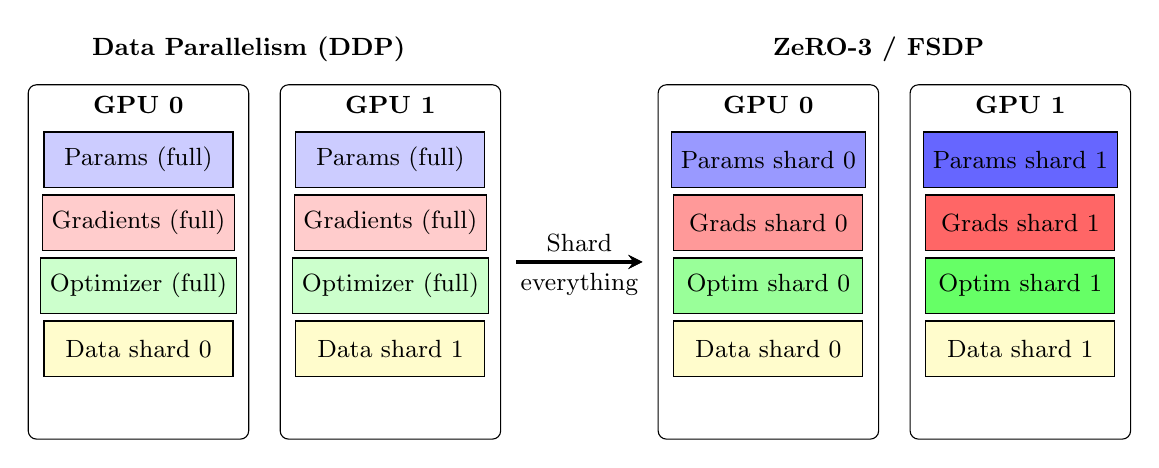
\begin{tikzpicture}[
    gpu/.style={rectangle, draw, minimum width=2.8cm, minimum height=4.5cm, rounded corners=3pt},
    mem/.style={rectangle, draw, minimum width=2.4cm, minimum height=0.7cm, font=\small},
    label/.style={font=\small\bfseries}
]
    % DDP
    \node[label] at (1.4, 5.2) {Data Parallelism (DDP)};

    % GPU 0
    \node[gpu] (g0) at (0, 2.5) {};
    \node[label] at (0, 4.5) {\small GPU 0};
    \node[mem, fill=blue!20] at (0, 3.8) {Params (full)};
    \node[mem, fill=red!20] at (0, 3.0) {Gradients (full)};
    \node[mem, fill=green!20] at (0, 2.2) {Optimizer (full)};
    \node[mem, fill=yellow!20] at (0, 1.4) {Data shard 0};

    % GPU 1
    \node[gpu] (g1) at (3.2, 2.5) {};
    \node[label] at (3.2, 4.5) {\small GPU 1};
    \node[mem, fill=blue!20] at (3.2, 3.8) {Params (full)};
    \node[mem, fill=red!20] at (3.2, 3.0) {Gradients (full)};
    \node[mem, fill=green!20] at (3.2, 2.2) {Optimizer (full)};
    \node[mem, fill=yellow!20] at (3.2, 1.4) {Data shard 1};

    % ZeRO-3 / FSDP
    \node[label] at (9.4, 5.2) {ZeRO-3 / FSDP};

    % GPU 0
    \node[gpu] (z0) at (8, 2.5) {};
    \node[label] at (8, 4.5) {\small GPU 0};
    \node[mem, fill=blue!40] at (8, 3.8) {Params shard 0};
    \node[mem, fill=red!40] at (8, 3.0) {Grads shard 0};
    \node[mem, fill=green!40] at (8, 2.2) {Optim shard 0};
    \node[mem, fill=yellow!20] at (8, 1.4) {Data shard 0};

    % GPU 1
    \node[gpu] (z1) at (11.2, 2.5) {};
    \node[label] at (11.2, 4.5) {\small GPU 1};
    \node[mem, fill=blue!60] at (11.2, 3.8) {Params shard 1};
    \node[mem, fill=red!60] at (11.2, 3.0) {Grads shard 1};
    \node[mem, fill=green!60] at (11.2, 2.2) {Optim shard 1};
    \node[mem, fill=yellow!20] at (11.2, 1.4) {Data shard 1};

    % Arrow between them
    \draw[very thick, ->, >=stealth] (4.8, 2.5) -- (6.4, 2.5) node[midway, above, font=\small] {Shard};
    \draw[very thick, ->, >=stealth] (4.8, 2.5) -- (6.4, 2.5) node[midway, below, font=\small] {everything};
\end{tikzpicture}
\caption{DDP stores full copies of everything on each GPU; ZeRO-3/FSDP shards parameters, gradients, and optimizer states, dramatically reducing per-GPU memory.}
\label{fig:ddp_vs_zero}
\end{figure}

%==============================================================================
\section{Training Debugging}
\label{sec:training_debug}
%==============================================================================

Training debugging is a core Staff-level skill. The loss curve tells you a story---you need to know how to read it.

\subsection{Loss Curve Diagnostics}

Refer to Figure~\ref{fig:loss_diagnostics} for the visual patterns. Here is the diagnostic playbook:

\begin{table}[H]
\centering
\caption{Training debugging: symptom to cause to fix}
\begin{tabularx}{\textwidth}{lXX}
\toprule
\textbf{Symptom} & \textbf{Likely Cause} & \textbf{Fix} \\
\midrule
Loss does not decrease at all & LR too low, bug in loss/data & Increase LR 10$\times$; verify labels match predictions; check model output shape \\
Loss decreases then plateaus & LR too low after initial phase; model capacity too small & Add LR schedule (cosine); increase model size; check data diversity \\
Loss oscillates wildly & LR too high; batch size too small & Reduce LR; increase batch; add gradient clipping \\
Loss spikes then recovers & Bad data batch; gradient explosion; LR schedule step & Add gradient clipping ($c = 1.0$); check data pipeline; lower LR \\
Loss goes to NaN & Numerical overflow; division by zero; LR far too high & Use mixed precision with loss scaling; add $\epsilon$ to divisions; reduce LR drastically \\
Train loss low, val loss high & Overfitting & Add dropout, weight decay, data augmentation; reduce model size; get more data \\
Train and val loss both high & Underfitting & Increase model capacity; train longer; increase LR; check data quality \\
\bottomrule
\end{tabularx}
\end{table}

\subsection{Gradient Statistics Monitoring}

Track per-layer gradient statistics during training:
\begin{itemize}
    \item \textbf{Gradient norm:} Should be roughly consistent across layers. If early layers have $10^{-6}$ and later layers have $10^{0}$, you have vanishing gradients.
    \item \textbf{Gradient mean:} Should be near zero (unbiased). A consistent nonzero mean suggests a data or label issue.
    \item \textbf{Update-to-weight ratio:} The ratio $\|\Delta\theta\| / \|\theta\|$ should be $\sim 10^{-3}$. Much larger means unstable training; much smaller means the model is barely changing.
\end{itemize}

\subsection{Learning Rate Finder}

\textbf{What it is.} Before training, sweep the LR from very small ($10^{-7}$) to very large ($10$) over a few hundred steps. Plot loss vs.\ LR. Pick the LR at the steepest descent (not the minimum---the minimum is already overshoot territory).

\textbf{Practical use.} Most useful for SGD. Less necessary for Adam, which is more robust to LR choice, but still helpful for sanity checking.

%==============================================================================
\section{Interview Questions}
\label{sec:training_interview}
%==============================================================================

\begin{interviewq}
\textbf{Q1: Your model's loss plateaus after initial descent. Walk through your debugging process.}

\textbf{What the interviewer is testing:} Systematic thinking, practical experience with training failures, ability to prioritize hypotheses from most to least likely.

\textbf{Strong answer:}

I would investigate in this order:

\begin{enumerate}
    \item \textbf{Check the learning rate schedule.} Is the LR already too small? Try increasing it or switching to cosine annealing with warm restarts. A plateau often means the current LR is too low to escape the current basin.

    \item \textbf{Check validation loss.} If validation loss is also plateaued (and still high), the model is underfitting---increase capacity or train longer. If validation loss is increasing while training loss plateaus, the model is at the edge of overfitting.

    \item \textbf{Examine gradient norms per layer.} Are early layers receiving gradients? Vanishing gradients cause effective early-layer freezing, which manifests as a plateau.

    \item \textbf{Check data.} Is the model seeing diverse batches, or is the data loader repeating patterns? Are there label noise issues capping achievable loss?

    \item \textbf{Try a larger model.} The current architecture may not have enough capacity for the task. Try doubling width or depth as a diagnostic.

    \item \textbf{Inspect the loss landscape.} Is the model stuck in a sharp local minimum? Increasing batch size or learning rate (or using SWA) can help escape sharp minima.
\end{enumerate}

\textbf{Common follow-ups:} ``How do you distinguish underfitting from a data quality ceiling?'' ``What if increasing LR causes divergence?'' ``How does batch size affect this?''
\end{interviewq}

\begin{interviewq}
\textbf{Q2: How would you scale training of a 70B parameter model across 256 GPUs?}

\textbf{What the interviewer is testing:} Understanding of distributed training strategies, ability to do back-of-the-envelope memory calculations, knowledge of modern training infrastructure.

\textbf{Strong answer:}

First, I would estimate memory requirements. A 70B model needs:
\begin{itemize}
    \item Parameters in BF16: $70\text{B} \times 2 = 140$ GB
    \item Optimizer states (AdamW, FP32): $70\text{B} \times 8 = 560$ GB (first + second moments)
    \item Gradients in BF16: $70\text{B} \times 2 = 140$ GB
    \item Total: $\sim 840$ GB, before activations
\end{itemize}

This does not fit on a single 80 GB A100. I would use a \textbf{3D parallelism} strategy:

\begin{enumerate}
    \item \textbf{Tensor parallelism (TP = 8):} Split each layer across 8 GPUs within a single node (connected via NVLink). This divides per-layer memory and compute by 8.

    \item \textbf{Pipeline parallelism (PP = 4):} Split the 80 Transformer layers into 4 stages of 20 layers each. Each stage runs on a different group of 8 GPUs. Use micro-batching to reduce the pipeline bubble.

    \item \textbf{Data parallelism (DP = 8):} The remaining $256 / (8 \times 4) = 8$ groups each run a data-parallel replica. Use ZeRO-1 to shard optimizer states across the 8 replicas.
\end{enumerate}

Additional optimizations: BF16 mixed precision, gradient checkpointing (to fit activations in memory), gradient accumulation if effective batch size needs to be larger than what the DP degree provides.

\textbf{Common follow-ups:} ``What is the pipeline bubble and how do you minimize it?'' ``How would you handle a node failure?'' ``What communication patterns does tensor parallelism require?''
\end{interviewq}

\begin{interviewq}
\textbf{Q3: Adam vs SGD with momentum---when would you pick each?}

\textbf{What the interviewer is testing:} Nuanced understanding of optimizer properties, not just memorized definitions. Ability to connect optimizer choice to task characteristics.

\textbf{Strong answer:}

\textbf{SGD with momentum} when: I am training a CNN on a well-studied task (ImageNet, object detection), have a known good training recipe, and care most about final generalization. SGD with a well-tuned cosine schedule consistently achieves better test accuracy on vision tasks, likely because the gradient noise from non-adaptive steps helps escape sharp minima and find flatter solutions.

\textbf{Adam(W)} when: I am training a Transformer, LLM, or any model where the loss landscape has highly variable curvature across parameters. Adam's per-parameter adaptive rate handles the heterogeneous gradient scales in attention layers (Q/K/V projections, embeddings, layer norms all have very different gradient magnitudes). Also better for: fast prototyping, GANs (where training is unstable), and any setting where I cannot afford extensive LR tuning.

\textbf{The nuanced point:} The performance gap between Adam and SGD has narrowed. AdamW with proper weight decay and cosine schedule now matches or beats SGD on many vision tasks (see ConvNeXt). The ``SGD generalizes better'' claim is mostly about Adam without proper decoupled weight decay.

\textbf{Common follow-ups:} ``Why does Adam sometimes generalize worse?'' ``What is the connection between adaptive learning rates and sharp minima?'' ``How does weight decay interact differently with each?''
\end{interviewq}

\begin{interviewq}
\textbf{Q4: Explain gradient accumulation and when you would use it.}

\textbf{What the interviewer is testing:} Understanding of the relationship between batch size, memory, and optimization; practical training knowledge.

\textbf{Strong answer:}

Gradient accumulation simulates a larger batch size without increasing GPU memory. Instead of updating parameters after every mini-batch, you:
\begin{enumerate}
    \item Forward and backward pass on mini-batch $i$, accumulate the gradient (add to running sum)
    \item Repeat for $k$ mini-batches (without zeroing gradients)
    \item After $k$ accumulations, divide by $k$ (average the gradients), then run the optimizer step
    \item Zero the gradients and repeat
\end{enumerate}

The effective batch size is $k \times B$ where $B$ is the per-step mini-batch size. Mathematically, this is equivalent to training with batch size $kB$ (the averaged gradient is identical), except that:
\begin{itemize}
    \item Batch normalization statistics are computed per mini-batch, not per effective batch (use LayerNorm/GroupNorm to avoid this issue)
    \item You get $k$ times fewer optimizer steps per epoch, so training is $k$ times slower in wall-clock time per update
\end{itemize}

\textbf{When I would use it:}
\begin{itemize}
    \item My GPU cannot fit the batch size required by a training recipe (e.g., a paper uses batch 2048 but I can only fit 256)
    \item Contrastive learning where larger batches improve performance (though note: for in-batch negatives like InfoNCE, accumulation does \textit{not} increase the effective negative count---you need true larger batches or techniques like gradient caching)
    \item Fine-tuning large models where even batch size 1 barely fits
\end{itemize}

\textbf{Common follow-ups:} ``Does gradient accumulation affect learning rate?'' (Yes---apply linear scaling to the effective batch size, not the mini-batch size.) ``How does it interact with mixed precision?'' (Accumulate in FP32 to avoid precision loss from many additions.)
\end{interviewq}